\documentclass{article}
\usepackage{kotex}
\usepackage{amssymb}
\usepackage{amsmath}
\usepackage{setspace}
\usepackage{graphicx}
\usepackage{booktabs}
\usepackage{subfigure}
\begin{document}
\setstretch{1.6}

\title{머신 러닝을 통한 신재생에너지 예측 최적화}
\author{18009 고도형}
\maketitle

\section{서론}
고객들의 필요에 따라 적절한 양의 에너지를 공급하기 위해 전력을 공급하는 회사들은 발전소의 생산율을 조절하고 다른 회사로부터 전력을 수입해서 수요를 충족시켜 왔다. 그러나 갈수록 필요한 전기에너지의 양이 증가하면서 수요가 전체 발전소의 생산량을 합한 것보다 큰 상황이 발생하는 것에 대비해 전력 시장에서 공급뿐만 아니라 수요를 조절하는 것도 필요해졌다. 그리하여 현재 전력 공급량에 맞추어 전기 사용자가 자신의 사용량을 변화시키는 수요 반응(DP; Demand Response)의 개념이 등장했다. 수요 반응은 현재 시장에서 제공 가능한 에너지의 양에 따른 인센티브를 제공하여 그에 따라 자연스럽게 소비자가 스스로의 전기 사용에 변화를 만드는 것을 말한다. 그리고 효율적인 에너지 사용을 위하여 도입된 스마트 그리드 시스템은 에너지를 절감하고 효율적으로 사용하기 위해 전력 시장에서 소비자의 능동적이고 자발적인 수요반응을 활용한다. 그리고 이를 위해 전력 수요를 상시 모니터링하며 수요의 증감에 따라 필요한 발전소의 발전량을 조절한다. 다행히 가정이나 공장의 전력 수요는 누적된 데이터를 통해 어렵지 않게 예측할 수 있고 전력을 수급하기 위한 발전소의 선택과 전력의 공급 시기를 정확히 만족시킬 수 있다. \newline
그런데 에너지의 초과수요를 방지하고 소비자로부터 수요 반응을 이끌어내기 위해서는 전력 수요뿐만 아니라 특정 시점에서의 한계 공급량이 어느 정도인지 미리 파악할 필요가 있다. 일반적인 화력 발전이나 원자력 발전의 경우에는 시간에 따른 발전량의 기복이 크지 않아 한계 공급량을 어렵지 않게 파악할 수 있으나 대부분의 신재생에너지는 기상 상황에 따라 발전량의 차이가 커 예측이 불가능하고 관리하기가 쉽지 않다. 이러한 신재생에너지의 발전량은 기상 파라미터 값과 깊은 연관성을 가지는 만큼 정확한 예측을 위해 주로 기상 데이터를 이용한 기계적 모델이 채택되고 있다.

\section{선행 연구}
Emil Isaksson과 Mikael Karpe Conde은 그들의 논문 Solar Power Forecasting with Machine Learning Techniques에서 머신 러닝 기반의 태양광 발전량 예측 모델을 설계하였다. 이 모델은 학습 알고리즘 중 하나인 인공신경망을 지도 학습의 도구로 활용하여 높은 정확도로 한계 공급량을 예측하였다. 연구진은 과거의 각종 기상 데이터들을 바탕으로 해당 환경 아래에서 실제 발전량과 근접하게 예측할 수 있는 모델을 훈련시키고 기상 예보 데이터를 접목시켜 전력 생산량을 예측하였다.

\section{ANN: Artificial Neural Network}
연구에 사용된 ANN 알고리즘은 인공 신경망(Artificial Neural Network)이라 불리는 학습 알고리즘이다. 정답과 비교해 가며 학습을 진행하는 지도학습과 데이터 클러스터링처럼 정답 없이 학습을 진행하는 비지도학습의 2가지 방법에 모두 적용될 수 있으나 해당 연구에서는 지도학습에 활용하였다. 인공신경망은 생물의 신경망에서 영감을 얻어 개발된 방법으로서 Node로서 구현되는 인공 뉴런을 모델링하여 문제 해결에 사용하는데 이는 일반적으로 독립 변수와 종속 변수 사이의 명확한 관계를 추측하기 어려운 함수를 추측하고 근사값을 추출하는데 유용하다. \newline
일반적으로 사용되는 기본적인 인공신경망 알고리즘인 다층인공신경망(Multi-Layer Neural Network)의 경우 다음과 같이 입력층(Input Layer), 은닉층(Hidden Layer), 그리고 출력층(Output Layer)로 구성된다. 각각의 Layer는 노드(Node)라고 불리는 뉴런들로 구성되어 있으며 이들을 연결하고 있는 구조가 바로 시냅스(Synapse)이다. 아래 Figure 1-(b)의 ANN은 입력층에 8개, 3개의 은닉층에 각각 9개씩, 그리고 출력층에 4개의 노드를 가지고 있다.

\begin{figure}[h]
\centering
\subfigure[Example of a Deep ANN]{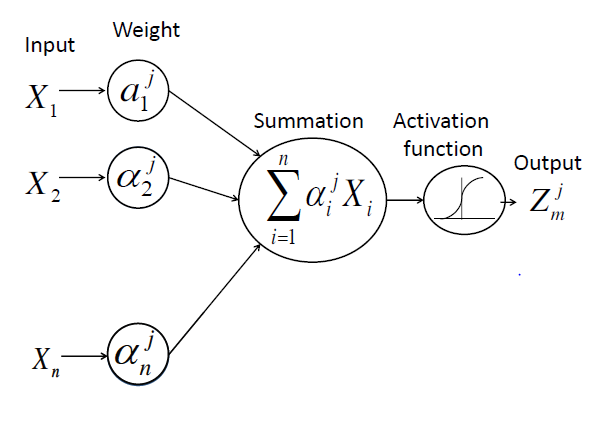
\includegraphics[width=0.3\textwidth]{./fig/Figure_1A.PNG}\hfill}
\subfigure[Visualization of a neuron]{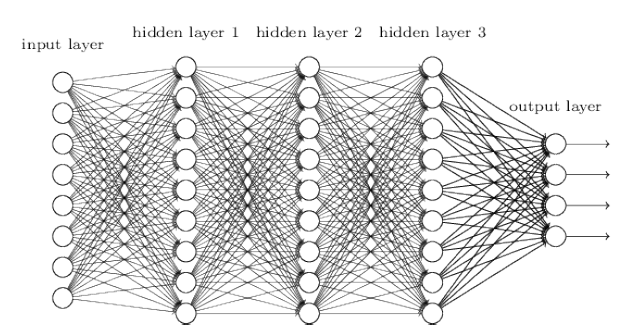
\includegraphics[width=0.4\textwidth]{./fig/Figure_1B.PNG}\hfill}
\caption{Mechanism of Artificial Neural Network}
\label{fig_1}
\end{figure}

입력층은 모델의 예측값을 도출하기 위한 시스템 외부로부터 독립 변수들을 입력받는 역할을 수행한다. 따라서 $n$개의 입력값을 받고자 한다면 입력층에 $n$개의 노드를 생성해야 한다. 다음으로 은닉층은 모든 입력 노드들로부터 독립 변수들의 입력값을 받아 각각의 노드에 존재하는 고유한 가중치를 적용한 합을 계산하고 이 값을 활성화 함수에 적용한다. 이제부터 뉴런과 파라미터를 동일하게 간주하고 전개하도록 하겠다.

\begin{figure}[h]
\centering
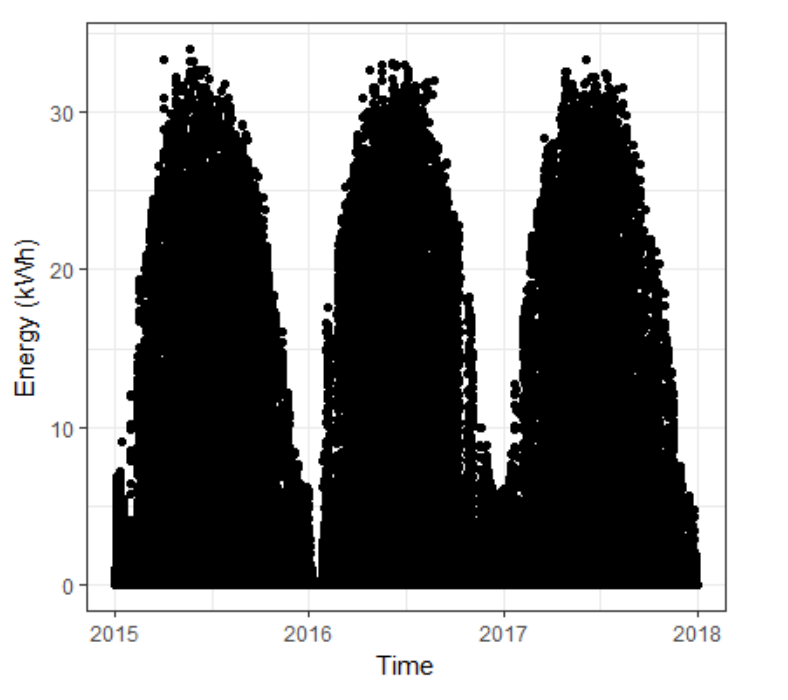
\includegraphics[scale=0.3]{./fig/Figure_2.png}
\caption{Simple ANN Model}
\label{fig_2}
\end{figure}

위 Figure 2에서 입력층에 사용된 $X_i^n$은 훈련 데이터 집합의 $i$번째 데이터의 $n$번째 파라미터를 의미한다. 또한, 은닉층을 표현하는데 사용된 $Z_m^j$는 입력층을 통과하여 $j$번째 은닉층에 도달한 데이터의 $m$번째 변형된 파라미터를 의미한다. 최종적인 값을 표현하는 출력층의 $y_n$은 추정 데이터의 $n$번째 파라미터를 의미한다. 이를 바탕으로 입력층의 뉴런과 이웃한 은닉층의 뉴런 사이에 전달되는 가중치의 합을 다음과 같이 표현할 수 있다.

\begin{equation}
Weight Sum = \sum_{k=1}^{n}(\alpha_k^j X_i^k)+b
\end{equation}

$\alpha_k^j$의 형태로 나타내어진 가중치는 은닉층을 이루는 하나의 뉴런과 입력층을 이루는 하나의 뉴런 사이에 형성되며 이는 두 레이어의 모든 뉴런에 대해 적용된다. 또한, 이 값은 초기에는 랜덤으로 주어졌다가 최적화 과정을 통해 예측값을 가장 잘 추정하는 값으로 조정된다. 가중치값은 은닉층으로 전송되기 전에 활성화 함수에 대입되고 그 출력값이 비로소 전송된다. 활성화 함수는 다양한 형태의 비선형함수가 사용되나 대표적으로는 시그모이드 함수, 하이퍼볼릭 탄젠트 함수, ReLU 함수 등이 이용된다. 다음은 차례로 각각의 함수를 표현한 것이다.

\begin{equation}
f(v)=\frac{1}{1+e^{-v}}
\end{equation}

\begin{equation}
f(v)=\frac{e^v-e^{-v}}{e^v+e^{-v}}
\end{equation}

\begin{equation}
f(v)=max[v,0]
\end{equation}

활성화 함수의 함숫값으로 표현된 변형된 파라미터값들은 이어지는 은닉층, 또는 출력층으로 전달하는 역할을 한다. 이때, 은닉층은 단 1개밖에 존재할 수 없는 출력층이나 입력층과 달리 여러 개가 존재할 수 있으며 2개 이상의 은닉층을 가지는 인공신경망을 특별히 Deep ANN이라 부른다. 이와 같이 인공신경망 네트워크가 구성되면 그 다음 목표는 각각의 뉴런과 시냅스가 가지는 가중치(Weight)와 편향(Bias)의 최적화로서 노드를 다시 되돌아가 업데이트하는 오차역전파 방법이 사용된다. 이 방법을 달성하기 위해 현재 상태의 오류를 판정할 수 있는 적절한 비용 함수를 세우고 Gradient Descent 방법이나 Levenberg-Marquardt 방법 등의 다양한 최적화 방법들을 적용하여 해결한다. 자세한 방법은 다루지 않겠다.

\section{교차검증: K-Fold Cross Validation}
검증 데이터 집합(Validation Dataset)은 훈련 데이터 집합(Training data set)으로 모델링을 시도할 때, 학습 상태를 점검하고 하이퍼파라미터를 조절할 수 있도록 하는 데이터 집합이다. 이러한 검증 데이터 집합은 일반적으로 훈련 데이터 집합에서 $n:m$ 비율로 나누어 사용하는데 이 연구에서는 하이퍼파라미터 중 하나인 인공신경망의 가중치와 편향 값을 탐색할 때 적용되었다.

\begin{figure}[h]
\centering
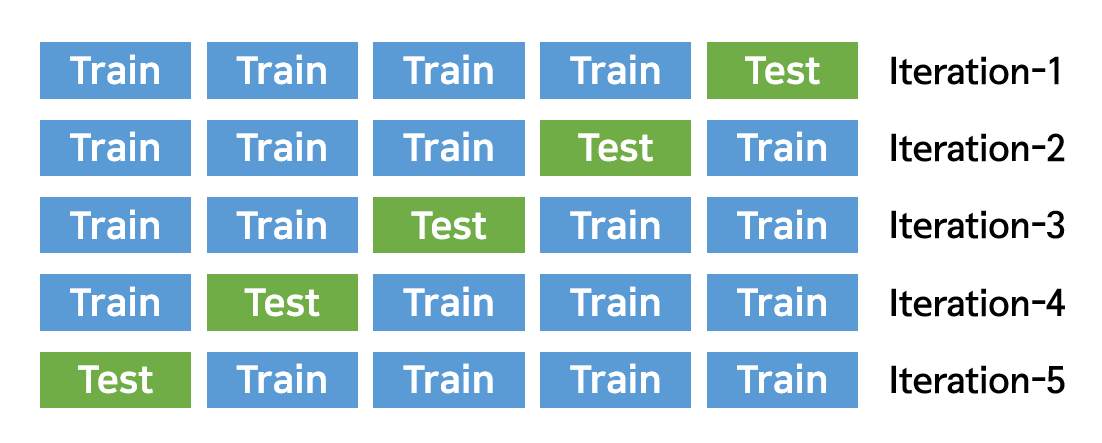
\includegraphics[scale=0.3]{./fig/Figure_3.png}
\caption{Process of Cross Validation}
\label{fig_1}
\end{figure}

아래 Figure 3에서 볼 수 있듯 총 5번의 훈련을 진행한다고 할 때, 각각의 훈련 단계(iteration)에서 훈련 데이터 집합을 5개의 부분집합으로 쪼개고 그 중 하나를 검증 데이터 집합으로 설정하여 알고리즘의 학습 상태를 점검하는 것을 알 수 있다. 연구에서 사용된 K-Fold Cross Validation 방법은 1개의 훈련 데이터 집합을 $K$개로 나누어 그 중 1개를 검증 데이터 집합으로, 나머지 $K-1$개를 훈련 데이터 집합으로 하여 모델을 학습시키는 것을 의미한다.

\section{데이터}
해당 연구에서는 모델을 훈련시키기 위해 다양한 형태의 기상 데이터들을 사용하였다. 연구가 스웨덴의 5개 지역에 대해 진행된 만큼 데이터 또한 각각의 지역에서 동일한 조건 아래 측정되었다. 우선, 2~3년에 걸쳐 측정한 파워 데이터는 고정된 태양광 PV 패널의 시간당 발전량을 kWh로 측정된 것이다. 이 데이터는 특정 기상 조건에서 실제 발전량을 나타내는 지표로 사용되었으며 모델의 추정값과 대조하여 그 오차를 줄이는 데 실질적으로 사용되었다.

\begin{figure}[h]
\centering
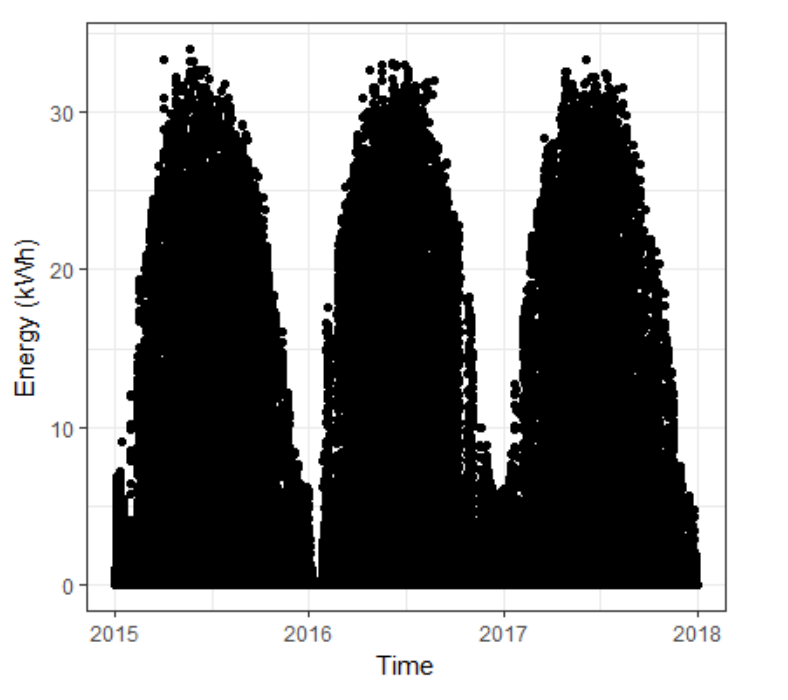
\includegraphics[scale=0.20]{./fig/Figure_4.png}
\caption{Energy Output for one of the 5 sites}
\label{fig_2}
\end{figure}

다음으로, 수치적 기상 예측 데이터(Numerical Weather Prediction Data)이다. Meteomatics의 API로부터 5개 지역의 2~3년 동안의 다양한 기상학적 변수들을 6시간마다 기록한 값을 얻었다. 이 데이터는 ANN의 입력층 파라미터로 설정되어 모델을 구현하는데 기여하였다. 자세한 정보는 Talbe 1을 참조하라.

\begin{table}[h]
    \begin{tabular}{@{}|c|c|c|@{}}
    \toprule
    \textbf{변수명}                & \textbf{NWP 데이터}                      & \textbf{단위} \\ \midrule
    total\_cloud\_cover : p     & 구름의 양                                 & \%          \\
    wind\_speed\_10m : ms       & 지상 10m 높이의 풍속                         & m/s         \\
    wind\_dir\_10m : d          & 지상 10m 높이의 풍향                         & m/s         \\
    t\_2m : C                   & 지상 2m 높이의 기온                          & C           \\
    clear\_sky\_rad : W         & Clear Sky Radiation                   & $W/m^2$     \\
    sfc\_pressure : hPa         & 기압                                    & hPa         \\
    diffuse\_rad : W            & 산란복사의 순간 Flux                         & $W/m^2$     \\
    global\_rad : W             & 전천복사의 순간 Flux                         & $W/m^2$     \\
    direct\_rad : W             & 직달 태양 복사의 순간 Flux                     & $W/m^2$     \\
    effective\_cloud\_cover : p & Effective Cloud Cover                 & \%          \\
    high\_cloud\_cover : p      & High Cloud Cover                      & \%          \\
    medium\_cloud\_cover : p    & Low Cloud Cover                       & \%          \\
    precip\_1h : mm             & 누적 강수량 (1시간)                          & mm          \\
    fresh\_snow\_1h : cm        & 누적 적설량 (1시간)                          & cm          \\
    global\_rad\_1h : J         & 누적 전천복사량 (1시간)                        & J           \\
    direct\_rad\_1h : J         & 누적 직달 태양복사량 (1시간)                     & J           \\
    diffuse\_rad\_1h : J        & 누적 산란복사량 (1시간)                        & J           \\
    cape : Jkg                  & Convective Available Potential Energy & J/kg of air \\
    relative\_humidity\_2m : p  & 지상 2m 지점의 상대 습도                       & \%          \\ \bottomrule
\end{tabular}
\caption{\label{tab:table_1}NWPs from Meteomatics}
\end{table}

\begin{figure}[!h]
\centering
\subfigure[A cloudy day]{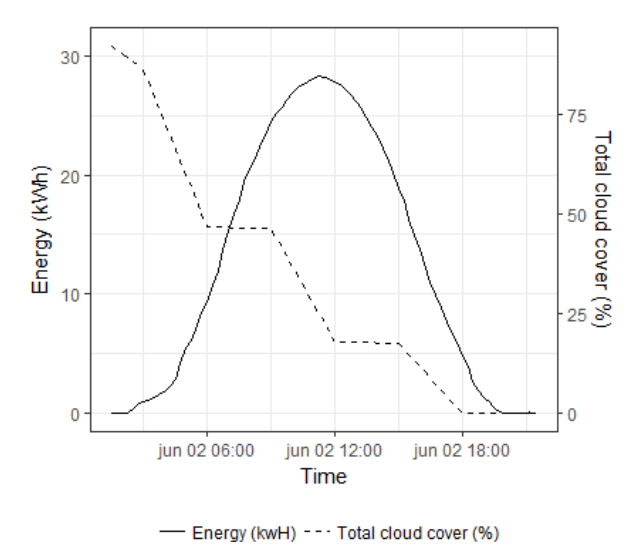
\includegraphics[width=0.45\textwidth]{./fig/Figure_5A.PNG}\hfill}
\subfigure[A sunny day]{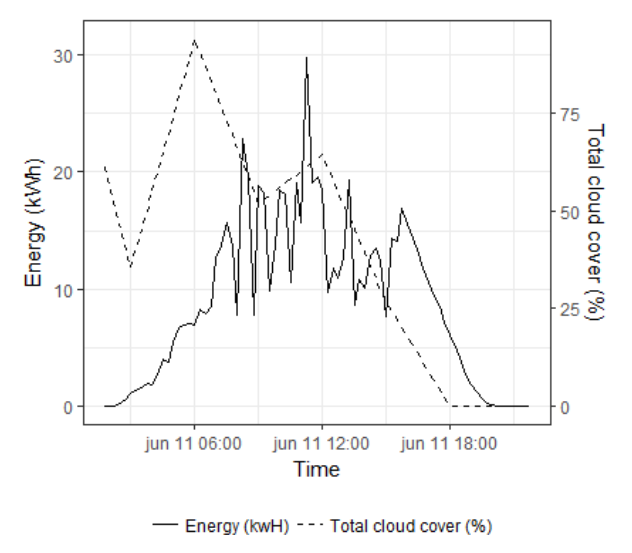
\includegraphics[width=0.45\textwidth]{./fig/Figure_5B.PNG}\hfill}
\caption{Correlation between NWP Data and Energy output}
\label{fig_3}
\end{figure}

Figure 5는 NWP 데이터 중 하나인 구름의 양(Total Cloud Cover)과 해당 조건에서의 서로 다른 두 태양광 PV 패널 사이의 발전량의 차이를 나타낸 그래프이다. 이처럼 Table 1의 다양한 변수를 파라미터로 하는 머신 러닝 모델을 구현함으로서 파라미터에 따른 예상 에너지 생산량을 최적화할 수 있다.

\section{인공신경망 모델의 구축}
추정값과 실제값 사이의 차이를 측정하기 위해 연구진은 아래의 평균 제곱근 오차(RMSE: Root Mean Squared Error)를 적용하였다.

\begin{equation}
RMSE=\sqrt{\frac{\sum_{i=1}^{n}(Y_i-\hat{Y_i})^2}{n}}
\end{equation}

$Y_i$는 실제 데이터의 값을, $\hat{Y_i}$는 예측한 데이터의 값을 나타낸다.
그리고 이를 바탕으로 다음과 같은 기상 데이터에 따른 발전량 예측 모델을 설계하였다. 해당 인공신경망 모델은 각각 10개의 노드를 갖춘 3개의 은닉층을 포함한 총 5개의 Layer와 시그모이드 활성화 함수를 채택하였다. Figure 2에서 볼 수 있듯, 연구진이 구현한 인공신경망 모델에서 입력층은 수집한 NWP 기상 데이터의 카테고리의 수, 10개이다. 즉, 특정 시간대에 발표된 기상 데이터를 이루는 각각의 파라미터값들을 입력층에 대입함으로서 출력층으로부터 1시간 간격으로 최대 5시간 후의 시간 당 발전량을 차례대로 추정한 데이터를 얻는 구조로 작동한다. 따라서 훈련 데이터 집합을 이루는 NWP 기상 데이터를 대입하고 이때 모델이 추정한 발전량과 앞서 조사한 파워 데이터를 비교하고 이때 발생한 오차를 비용 함수에 대입하여 이를 다양한 방법으로 최적화하는 과정을 거치며 인공신경망 모델을 보다 정확한 예측을 할 수 있도록 훈련시키는 것이다. Forecast Horizon은 입력받은 데이터를 기준으로 몇 시간 후의 태양광 PV 패널의 전력 생산량을 예측할 것인지를 결정하는 파라미터로 해당 연구에서는 15분에서 5시간까지 1시간 간격으로 설정하였다. 연구진은 결과를 평가할 수 있는 테스트 데이터 집합으로 2017년의 NWP 기상 데이터를 활용하였다. 이 테스트 데이터 집합은 훈련이 완료된 인공신경망 모델에 대입하여 데이터가 발표된 시점을 기준으로 1-5시간 내의 태양광 PV 패널의 시간당 에너지 생산량을 효과적으로 예측하는데 사용된다.

\section{결과}


\section{결론}

\end{document}